\documentclass{article}
\usepackage[utf8]{inputenc}
\usepackage[T1]{fontenc}
\usepackage[ngerman]{babel}
\usepackage[
    left = \glqq{},% 
    right = \grqq{},% 
    leftsub = \glq{},% 
    rightsub = \grq{} %
]{dirtytalk}
\usepackage{graphicx}
\graphicspath{ {./assets/} }
\usepackage{multicol}

\title{FSST}
\author{Felix Hofinger}
\date{October 2022}

\setcounter{secnumdepth}{4}
\setcounter{tocdepth}{4}

\begin{document}

\maketitle
\newpage
\tableofcontents
\newpage

\section{Exception Handling}

Exceptions sind Objekte:
\begin{itemize}
    \item Felder: Informationen über den Fehler
    \item Methoden: Ausgabe der Fehlerinformationen, etc.
\end{itemize}

\vspace{1em}
\begin{verbatim}
try {
    ...
    p();
    ...
} catch (Exception e) {
    System.out.println(e.toString());
}
\end{verbatim}
\begin{verbatim}
void p() throws Exception {
    ...
    throw new Exception();
    ...
}
\end{verbatim}

\begin{table}[!htbp]
    \centering
    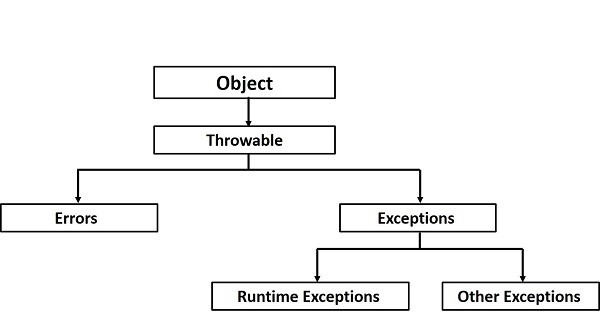
\includegraphics[scale=0.5]{1/exception_hierarchy.jpg}
    \caption{Exception Hierarchy}
    \label{tab:exception_hierarchy}
\end{table}

\begin{verbatim}
    try {
        ...
    } catch(MyException e) { // fängt MyException u. U.
    } catch(Exception e) { // fängt Exception u. U.
    } catch(Throwable e) { // fängt alle Exceptions
    }
\end{verbatim}


\section{Prozesse}

\begin{itemize}
    \item Ablauf eines sequentiellen Programms
    \item Kontext / Prozessumgebung
    \item Betriebssysteme, die Programme mit mehreren parallel ausführbaren Programmauschnitten zulassen. \\
          \hspace*{2em} -> Threads
\end{itemize}

\newpage
\subsection{Eigenschaften}

\begin{itemize}
    \item Aus Sicht des Betriebssystems: Objekte die die CPU Kapazität zugeteilt bekommen
    \item Multitasking Betriebssystem: mehrere Prozesse gleichzeitig im Speicher \\
          \hspace*{2em} Bei ein-Prozessor System: \\
          \hspace*{4em} -> immer nur ein Prozess aktiv \\
          \hspace*{4em} -> ständig zwischen Prozessen wechseln \\
          \hspace*{4em} -> quasi-paralleler Ablauf
    \item Parallel bzw. quasi-paralleler Ablauf -> nebenläufigkeit
    \item Zustand
    \item Kontext: CPU Register, Ressourcen (Arbeitsregister, Dateien, ...)
    \item "Kinderprozesse" -> Prozessbäume
    \item Prozesse können miteinander kommunizieren \\
          \hspace*{2em} -> Interprozesskommunikation
    \item Prozesse können voneinander abhängen \\
          \hspace*{2em} -> kooperierende Prozesse \\
          \hspace*{2em} -> Suchorganisation
    \item Prioritat
\end{itemize}

\subsection{Repräsentation von Prozessen}

\begin{itemize}
    \item für jeden Prozess gibt es einen Prozess-Struktur-Block (PCB)
    \item PCB: Prozess-ID, Priorität, Status, Kontext, ... \\
          \hspace*{2em} -> werden in verketteter Liste verwaltet (Prozesstabelle)
\end{itemize}

% TODO: ADD IMAGE

Zuteilung der CPU an einen bereiten Prozess macht der Scheduler. \\
\hspace*{3em} -> unterschiedliche Strategien

Prozesswechesel:
\begin{itemize}
    \item[1,] Retten des Prozesskontext
    \item[2,] Aktivieren des neuen Kontext
    \item[3,] PCB und Wakelist aktualisieren \\
        \hspace*{2em} -> anderer Prozess läuft weiter
\end{itemize}

\subsection{Process-Scheduler}

\begin{itemize}
    \item macht nur bei Multitasking Systemen Sinn
    \item wählt aus der Liste von bereiten Prozessen den nächsten aktiven Prozess aus
    \item Zeitpunkte: \\
          \hspace*{2em} -> Erzeugung neuer Prozesse \\
          \hspace*{2em} -> Beendung eines Prozesses \\
          \hspace*{2em} -> Blockierung des aktiven Prozesses \\
          \hspace*{2em} -> Unterbrechung durch I/O-Gerät \\
          \hspace*{2em} -> Unterbrechung durch Timer \\
\end{itemize}

\subsubsection{Ziele des Schedulers}

\begin{itemize}
    \item Entscheiden, wer \say{rechnen} darf
    \item Scheduling Algorithmus
    \item Gerechtigkeit
    \item Effizienz
    \item Antwortzeit
    \item Verweilzeit
    \item Durchsatz
    \item Terminerfüllung
\end{itemize}

\subsubsection{Grundsysteme für Scheduling}

\begin{multicols}{2}
    \center{kooperatives Multitasking \\ non-preemptive}
    \begin{itemize}
        \item aktiver Prozess gibt CPU freiwillig her
        \item geringer Verwaltungsaufwand \\
              \hspace*{1em} -> Gefahr: Blockierung durch
              \hspace*{2.5em} unkooperativen Prozess
    \end{itemize}
    \columnbreak

    \center{verdrängendes Multitasking \\ preemptive}
    \begin{itemize}
        \item dem aktiven Prozess wird die CPU vom Scheduler entzogen (z.B. nach Zeit ablauf -> Timer interrupt)
        \item hoher Verwaltungsaufwand
        \item kein Blockieren
    \end{itemize}
\end{multicols}

\subsubsection{Strategien}

\paragraph{Eingangsreihenfolge (first come, first serve)}
\begin{itemize}
    \item Zuteilung d. CPU in Startreihenfolge
    \item neue Prozesse \say{hinten anstellen}
    \item Wechsel: Prozess fertig \underline{oder} blockiert
    \item[->] non-preemptive
    \item[->] super Systemauslastung
    \item[->] schlechtes Antwort- Zeitverhältnis
    \item[->] einfach
\end{itemize}

\paragraph{Kürzester Job zuerst (shortest job first)}
\begin{itemize}
    \item Zuteilung d. CPU nach bekannter/geschätzter Rechenzeit d. Prozesse
\end{itemize}

\paragraph{Zeitscheibenverfahren (round robin)}
\begin{itemize}
    \item CPU wird zyklisch nacheinander allen bereiten Prozessen für eine bestimmte Zeit zugeordnet
    \item[->] preemptive
    \item[->] alle haben gleiche Priorität
\end{itemize}

\paragraph{Prioritätssteuerung}
\begin{itemize}
    \item Jeder Prozess hat Priorität
    \item vergabe der CPU in absteigender Priorität
    \item Prozess mit niedriger Priorität bekommt die CPU erst dann, wenn alle Prozesse mit höherer Priorität fertig sind
    \item Ein bereit-werdender Prozess mit höherer Priorität als aktiver Prozess \\
          \hspace*{2em} -> verdrängt den aktiven Prozess
\end{itemize}

\end{document}